\chapter{Fermat's Little Theorem and its Consequences}\label{chapter:modular-arithmetic}

\section{Fermat's Little Theorem}

\begin{theorem}[Fermat's Little Theorem]\label{theorem:fermats-little-theorem}
  Consider a prime number $p$ and an integer $a$. Then the congruence
  \begin{equation*}
    a^{p}\equiv a\pmod{p}
  \end{equation*}
  holds.
\end{theorem}

\begin{remark}
  Note that the congruence $(-a)^p\equiv -a^p\pmod{p}$ holds for all primes $p$, so it suffices to prove the claim for the nonnegative integers.
\end{remark}

\begin{proof}[Fermat's additive proof]
  This proof is by induction on $a$. The base case $0^p\equiv 0\pmod{p}$ clearly holds.

  For the inductive step, assume that $a^p\equiv a\pmod{p}$. \zcrefnamed{theorem:binomial-theorem} then gives us that
  \begin{equation*}
    (a+1)^p=\sum_{k=0}^p \binom{p}{k}a^k
  \end{equation*}
  However, note that $p\mid\binom{p}{k}$ for any $0<k<p$. We therefore find that
  \begin{equation*}
    (a+1)^p\equiv a^p+1\pmod{p}.
  \end{equation*}
  Since $a^p\equiv a\pmod{p}$ holds by the induction hypothesis, the claim follows.
\end{proof}

\begin{figure}[t]
  \centering
  \begin{subfigure}{0.45\textwidth}
    \centering
    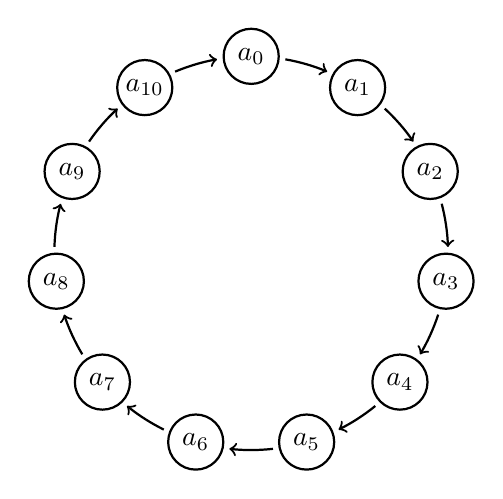
\begin{tikzpicture}[
      thick, every node/.style={circle, draw, minimum size=7mm, inner sep=1pt}]
      \def\n{11}
      \def\radius{2.5cm}
      
      \foreach \i in {1,...,\n} {
        \pgfmathsetmacro{\value}{int(\i-1)}
        \node (N\i) at ({90-360/\n*(\i-1)}:\radius) {$a_{\value}$};
      }
      
      \foreach \i in {1,...,\n} {
        \pgfmathsetmacro{\angle}{90-360/\n*(\i-1)}
        \draw[->] 
        (\angle-10:\radius)
        arc[start angle=\angle-10, delta angle=-360/\n+20, radius=\radius];
      }
    \end{tikzpicture}  

  \end{subfigure}
  \hfill
  \begin{subfigure}{0.45\textwidth}
    \centering
    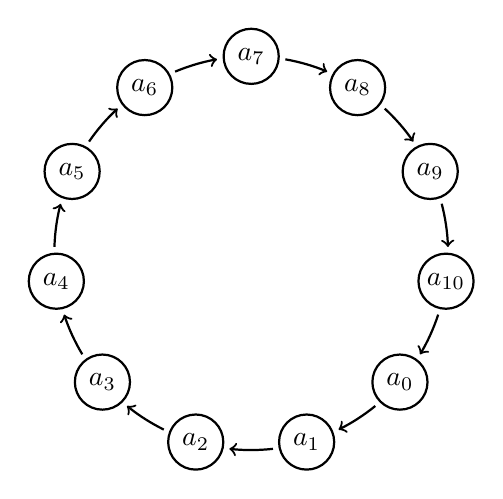
\begin{tikzpicture}[
      thick, every node/.style={circle, draw, minimum size=7mm, inner sep=1pt}]
      \def\n{11}
      \def\radius{2.5cm}
      
      \foreach \i in {1,...,\n} {
        \pgfmathsetmacro{\value}{int(mod(\n+\i-5,\n))}
        \node (N\i) at ({90-360/\n*(\i-1)}:\radius) {$a_{\value}$};
      }
      
      \foreach \i in {1,...,\n} {
        \pgfmathsetmacro{\angle}{90-360/\n*(\i-1)}
        \draw[->] 
        (\angle-10:\radius)
        arc[start angle=\angle-10, delta angle=-360/\n+20, radius=\radius];
      }
    \end{tikzpicture}  
  \end{subfigure}
  \caption[Golomb's proof of Fermat's Little Theorem]{\label{figure:golombs-proof-FLT}In Golomb's proof of Fermat's Little Theorem, two labellings of a cyclic set $C$ with elements from a set $A$ are considered the same---or equivalent---if one can be obtained from the other by rotation.}
\end{figure}

\begin{proof}[Golomb's combinatorial proof \cite{golomb1956}]
  Consider a set $A$ with $a$ elements, and a cyclic set $C$ with $p$ elements. There are $a^p$ functions from $C$ to $A$. Each such function $f:C\to A$ can be viewed as a labelling of each of the elements of $C$ by an element of $A$.

  Since the set $C$ is cyclically ordered, it is natural to consider two such labellings equivalent if one can be obtained from the other by rotating the cyclic set $C$. We indicated this equivalence in \zcref{figure:golombs-proof-FLT}. We claim that the number of functions that are equivalent to a labelling $f$ is always a divisor of the number of elements of $C$, which is $p$. Indeed, if $s:C\to C$ is the one-step rotation, then the number of functions equivalent to $f$ is equal to the least positive integer $k$ such that
  \begin{equation*}
    f\circ s^k=f.
  \end{equation*}
  Moreover, since $s^p$ is the identity on $C$, we always have $f\circ s^p=f$, and therefore $k\mid p$. By the assumption that $p$ is prime, there are two possibilities:
  \begin{enumerate}
  \item In the first case, $f$ is the only function equivalent to itself. This is the case if and only if $f$ is constant.
  \item In the second case, there are exactly $p$ functions equivalent to $f$, including $f$ itself. This is the case if and only if $f$ is nonconstant.
  \end{enumerate}
  Now note that the number of constant functions from $C$ to $A$ is exactly $a$. The number of nonconstant functions is therefore $a^p-a$. Since the nonconstant functions are partitioned into equivalence classes of size $p$, it follows that $a^p-a$ is divisible by $p$.
\end{proof}

\begin{corollary}
  Consider a prime number $p$ and an integer $a$ not divisible by $p$. Then the congruence
  \begin{equation*}
    a^{p-1}\equiv 1\pmod{p}
  \end{equation*}
  holds.
\end{corollary}

\begin{proof}
  Since $a$ is not divisible by $p$, it follows that $a$ is relatively prime to $p$, and therefore the claim follows from the cancellation law
  \begin{equation*}
    ax\equiv ay\pmod{p}\qquad\Rightarrow\qquad x\equiv y\pmod{p}.\qedhere
  \end{equation*}
\end{proof}

Fermat's Little Theorem can be used to analyze the prime divisors of special numbers such as Fermat numbers or Mersenne numbers. Regarding Fermat numbers, we have the following theorem, which is of great help when trying to prove or disprove that a Fermat number is prime.

\begin{theorem}\label{theorem:prime-divisors-fermat-numbers}
  If $p$ is a prime divisor of a Fermat number $F_n:=2^{2^n}+1$, then
  \begin{equation*}
    p\equiv 1\pmod{2^{n+1}}.
  \end{equation*}
\end{theorem}

\begin{proof}
  If $p$ is a prime divisor of $2^{2^n}+1$, then it follows that
  \begin{equation*}
    2^{2^n}\equiv -1\pmod{p}.
  \end{equation*}
  This implies via \zcrefnamed{theorem:order-theorem} that $\ord_p(2)\mid 2^{n+1}$. In particular, $\ord_p(2)=2^k$ for some number $k\leq n+1$. However, note that
  \begin{equation*}
    2^{2^k}\equiv 1\pmod{p}\qquad\text{implies}\qquad 2^{2^{k+1}}= (2^{2^k})^2\equiv 1 \pmod{p}.
  \end{equation*}
  Since $2^{2^{n}}\equiv -1\pmod{p}$, it follows that the order of $2$ modulo $p$ cannot divide $2^n$. Thus, it follows that $\ord_p(2)=2^{n+1}$. By \zcrefnamed{theorem:fermats-little-theorem}, we conclude that
  \begin{equation*}
    2^{n+1}\mid p-1.\qedhere
  \end{equation*}
\end{proof}

\begin{corollary}\label{corollary:F4}
  The fourth Fermat number $2^{2^4}+1=65537$ is prime.
\end{corollary}

\begin{proof}
  Any prime divisor of $F_4=2^{2^4}+1$ must satisfy the congruence $p\equiv 1\pmod{33}$. If $F_4$ is composite, then it must have a prime divisor below $\sqrt{F_4}$, and thus below $2^8=256$. The sieve of Eratosthenes displayed in \zcref{figure:sieve-of-eratosthenes} reveals that the only two primes $p\equiv 1\pmod{33}$ below $256$ are $97$ and $193$. A quick computation gives that
  \begin{equation*}
    F_4\equiv 62\pmod{97}\qquad\text{and}\qquad F_4\equiv 110\pmod{193},
  \end{equation*}
  so that neither $97$ nor $193$ is a prime divisor of $F_4$, and therefore we conclude that $F_4$ is prime.
\end{proof}

\begin{corollary}\label{corollary:F5}
  The fifth Fermat number $2^{2^5}+1=4,294,967,297$ is composite, and its smallest prime factor is $641$.
\end{corollary}

\begin{proof}
  By \zcref{theorem:prime-divisors-fermat-numbers} it follows that any prime divisor of $2^{2^5}+1$ must satisfy
  \begin{equation*}
    p\equiv 1\pmod{2^6}.
  \end{equation*}
  The prime numbers of the form $64k+1$ below one thousand are $193$, $257$, $449$, $577$, and $641$, as can be read off of \zcref{figure:sieve-of-eratosthenes}. We will prove that $193$, $257$, $449$, and $577$ do not divide $F_5$, and that $641$ does.
  \begin{enumerate}
  \item First, we note that $3\cdot 2^6\equiv -1\pmod{193}$, which implies that
    \begin{equation*}
      3\equiv -2^{-6}\pmod{193}.
    \end{equation*}
    A quick computation shows that $3^2=9$, $3^4=81=2^6+2^4+1$, and $3^8=6561=34\cdot 193-1$, so that
    \begin{equation*}
      3^8\equiv -1\pmod{193}
    \end{equation*}
    and thus $\ord_{193}(3)=16$. It follows that
    \begin{equation*}
      1\equiv 3^{16}\equiv (-2)^{6\cdot 16}\equiv 2^{96}\pmod{193},
    \end{equation*}
    which allows us to conclude that $\ord_{193}(2)\mid 96$. Now observe that if $193\mid F_5$ so that $2^{32}\equiv -1\pmod{193}$, then we'd have $\ord_{193}(2)=64\nmid 96$, a contradiction.
  \item Note that $257$ is itself a Fermat number. In \zcrefnamed{theorem:goldbachs-theorem} we showed that any two distinct Fermat numbers are relatively prime, so that $257\nmid F_5$.
  \item To show that $449\nmid 2^{32}+1$, we will simply compute $2^{32}\pmod{449}$. Note that $2^9\equiv 2^6-1\pmod{449}$. This allows us to compute
    \begin{align*}
      2^{16}
      & \equiv 2^7(2^6-1) \\
      & \equiv 2^{13}-2^7 \\
      & \equiv 2^4(2^6-1)-2^7 \\
      & \equiv 2^{10}-2^7-2^4 \\
      & \equiv 2(2^6-1)-2^7-2^4 \\
      & \equiv -2^4-2\pmod{449}.
    \end{align*}
    It follows that $2^{32}\equiv (-2^4-2)^2\equiv 2^8+2^6+2^2\equiv 324\pmod{449}$, so we see that $2^{32}\nequiv-1\pmod{449}$.
  \item Here we note that $2^9\equiv -(2^6+1)\pmod{577}$. By a similar calculation as above, we compute that
    \begin{equation*}
      2^{32}\equiv -2^8-2^5-2\equiv 287\pmod{577}.
    \end{equation*}
    Since $2^{32}\nequiv-1\pmod{577}$, it follows that $577\nmid F_5$.
  \item Finally, we prove that $641\mid F_5$. Euler's insight was that $641=5^4+2^4$, so that
    \begin{equation*}
      5^4\equiv -2^4\pmod{641}.
    \end{equation*}
    Furthermore, we have $641=5\cdot 2^7+1$, so that $5\equiv -2^{-7}\pmod{641}$. It follows that
    \begin{equation*}
      2^{32}\equiv 2^4\cdot 2^{7\cdot 4}\equiv -5^4\cdot 2^{7\cdot 4}\equiv -(5\cdot 2^7)^4\equiv - (-1)^4\equiv -1 \pmod{641}.
    \end{equation*}
    We conclude that $641\mid 2^{32}+1$.\qedhere
  \end{enumerate}
\end{proof}

\begin{remark}
  \'Edouard Lucas showed that any prime divisor $p\mid F_n$ of the $n$\supth Fermat number $F_n$, where $n\geq 2$, must in fact be of the form $k2^{n+2}+1$. Had Euler known this stronger restriction on the prime divisors of the Fermat numbers, he wouldn't even have to cover the cases $193$, $449$, and $577$!
\end{remark}

\section{Euler's Theorem}

Euler figured out a way to generalize Fermat's Little Theorem to the composite moduli. He made use of his totient function $\phi$, which counts for each $n$ the number of $0\leq m<n$ relatively prime to $n$.

\begin{theorem}[Euler's Theorem]\label{theorem:eulers-theorem}
  Consider a natural number $n$ and an integer $a$ such that $\gcd(a,n)=1$. The congruence
  \begin{equation*}
    a^{\phi(n)}\equiv 1\pmod{n}
  \end{equation*}
  holds
\end{theorem}

We present two proofs of Euler's Theorem. The first is the standard proof, and the other is inspired by methods of group theory.

\begin{proof}[First proof of Euler's Theorem]
  Consider an integer $a$ relatively prime to $n$, and consider a reduced residue system $r_1,\ldots,r_{\phi(n)}$ modulo $n$. We claim that
  \begin{equation*}
    ar_1,\ldots,ar_{\phi(n)}
  \end{equation*}
  is again a reduced residue system modulo $n$. Indeed, since multiplying by $a$ induces a bijection on $\mathbb{Z}/n\mathbb{Z}$, we see that all integers $ar_1,\ldots,ar_{\phi(n)}$ are incongruent. Furthermore, the product of any two integers relatively prime to $n$ is again relatively prime to $n$, so all the integers $ar_i$ are relatively prime to $n$. Since any set of $\phi(n)$ incongruent integers relatively prime to $n$ form a reduced residue system, the claim follows.

  Using that the integers $ar_1,\ldots,ar_{\phi(n)}$ form a reduced residue system, it follows that
  \begin{equation*}
    \prod_{i=1}^{\phi(n)}r_i\equiv \prod_{i=1}^{\phi(n)}ar_i = a^{\phi(n)}\prod_{i=1}^{\phi(n)}r_i\pmod{n}
  \end{equation*}
  Since $\prod_{i=1}^{\phi(n)}r_i$ is relatively prime to $n$, it follows that $a^{\phi(n)}\equiv 1\pmod{n}$.
\end{proof}

\begin{proof}[Second proof of Euler's Theorem]
  Consider the least positive integer $k$ such that $a^k\equiv 1\pmod{n}$, and consider the relation $\sim$ on the set of integers $0\leq b<n$ relatively prime to $n$, where
  \begin{equation*}
    b\sim c \qquad\text{if and only if}\qquad \exists_{0\leq i< k} ba^i\equiv c\pmod{n}.
  \end{equation*}
  This relation is reflexive, because $ba^0 \equiv b\pmod{n}$. It is symmetric, because if $ba^i\equiv c\pmod{n}$ for some nonzero $i$, then $ca^{k-i}\equiv ba^ia^{k-i}\equiv b\pmod{n}$. Furthermore, it is transitive, because if $ba^i\equiv c$ and $ca^j\equiv d$, then $ba^{i+j}\equiv d$. If $k\leq i+j$, then we find that also $ba^{i+j-k}\equiv d$. Thus, the relation $\sim$ is an equivalence relation.

  We claim that each equivalence class has size $k$. Indeed, for each $b$, the set
  \begin{equation*}
    \{b,ba,ba^2,\ldots,ba^{k-1}\}
  \end{equation*}
  consists of $k$ distinct elements, because multiplying with $b$ is a bijection. Thus we have partitioned the set of all numbers $0\leq b<n$ relatively prime to $n$ into equivalence classes of size $k$. On the other hand, the total number of elements $0\leq b<n$ relatively prime to $n$ is the number $\phi(n)$. This shows that $k\mid \phi(n)$, so it follows that $a^{\phi(n)}\equiv 1\pmod{n}$.
\end{proof}

\begin{remark}
  The second proof of Euler's theorem can be simplified using the language of group theory. A \emph{group} is a set $G$ equipped with a binary operation $x,y\mapsto xy$, a unary operation $x\mapsto x^{-1}$, and a unit element $1$, satisfying the axioms
  \begin{align*}
    (xy)z & = x(yz) \\
    x1 & = x \\
    1x & = x \\
    xx^{-1} & = 1 \\
    x^{-1}x & = 1.
  \end{align*}
  One can show that the set of integers modulo $n$ relatively prime to $n$ forms a group, where the binary operation is multiplication, the unit element is the integer $1$, and the inverse $x^{-1}$ of an integer $x$ modulo $n$ is the unique solution to the equation $xy\equiv 1\pmod{n}$. The number of elements in this group is $\phi(n)$. For any integer $a$ modulo $n$ relatively prime to $n$ such that $a^k\equiv 1\pmod{n}$, the set $\{1,a,a^2,\ldots,a^{k-1}\}$ is a subgroup, which means that it is closed under the group operations. The argument where we introduced an equivalence relation $\sim$ to partition the set of all integers modulo $n$ relatively prime to $n$ into equivalence classes of size $k$ is an instance of a much more general result, Lagrange's Theorem, which asserts that the size of any subgroup of a finite group divides the size of the entire group.
\end{remark}

Since $\phi(p)=p-1$, it follows that \zcrefnamed{theorem:fermats-little-theorem} is also a direct corollary of \zcrefnamed{theorem:eulers-theorem}.

\begin{remark}
  We saw the multiplicative order featuring in the second proof of \zcrefnamed{theorem:eulers-theorem}. Thus, using the second proof of Euler's theorem we immediately observe that
  \begin{equation*}
    \ord_n(a)\mid \phi(n),
  \end{equation*}
  for any $a$ and $n$ such that $\gcd(a,n)=1$.
\end{remark}

Some questions about Euler's totient function remain unresolved. While we have seen that $\phi(p)=p-1$ for any prime number $p$, Lehmer asked whether there is any composite number $n$ such that
\begin{equation*}
  \phi(n)\mid n-1.
\end{equation*}
This open problem is now known as \emph{Lehmer's problem} \cite{lehmer1933}.

\section{Wilson's Theorem}

The following theorem is a factorial criterion by which to decide whether a number is prime. It states that $n$ is prime if and only if the congruence
\begin{equation*}
  (n-1)!\equiv -1\pmod{n}
\end{equation*}
holds.

In the European mathematical tradition, it was first published by Edward Waring, who attributed it as follows to John Wilson \cite[p.~380]{waring1782} along with high praise: \textit{This most elegant property of prime numbers was discovered by the most illustrious and most skilled mathematician, John Wilson, Esquire.} However, neither Wilson nor Waring were able to rigorously prove this property of the prime numbers. The first to give a proof was Joseph--Louis Lagrange \cite{lagrange1771}. Euler, and later Gauss, gave separate proofs of this fact.

\begin{theorem}[Wilson's Theorem]\label{theorem:wilsons-theorem}
  A natural number $n\geq 2$ is prime if and only if
  \begin{equation*}
    (n-1)!\equiv -1 \pmod{n}.
  \end{equation*}
\end{theorem}

\begin{proof}
  First, we observe that the claim holds for $n=2$, since $1\equiv -1\pmod{2}$.
  
  Suppose that $n$ is prime strictly greater than $2$. Then every integer $0<a<n$ has a multiplicative inverse modulo $n$, meaning that for every integer $a$ there is an integer $a^{-1}$ such that
  \begin{equation*}
    aa^{-1}\equiv 1.
  \end{equation*}
  Now we group the integers $1\leq a < n$ into pairs with their inverses. 
  By \zcref{exercise:self-inverse-modulo-prime} and the assumption that $n\neq 2$, there are exactly two integers that would pair up with themselves because they are their own inverses: The integers $1$ and $-1$ are the only two integers $a$ modulo $n$ for which the congruence $a^2\equiv 1\pmod{n}$ holds. The other integers come in proper pairs $(a,a^{-1})$. Therefore, we have
  \begin{equation*}
    (n-1)!\equiv 1(n-1)\equiv -1\pmod{n}.
  \end{equation*}

  Conversely, suppose that the congruence $(n-1)!\equiv -1\pmod{n}$ holds. Since any $0<a<n$ is a divisor of $(n-1)!$, it follows that for any such $a$ there is a solution to the linear congruence
  \begin{equation*}
    ax\equiv -1\pmod{n}.
  \end{equation*}
  This implies that any $0<a<n$ is invertible modulo $n$, so it follows that $\gcd(a,n)=1$ for all $0<a<n$. We conclude that the only proper divisor of $n$ is $1$, and therefore $n$ is prime.
\end{proof}

\begin{proof}[Second proof of the forward direction of \zcrefnamed{theorem:wilsons-theorem}] Consider a prime $p$, and consider the monic polynomial \begin{equation*} f(x)=\prod_{k=0}^{p-1}(x-k). \end{equation*} Since every element is a root of $f(x)$ modulo $p$, it follows by \zcrefnamed{theorem:fermats-little-theorem} that $f(x)\equiv x^p-x\pmod{p}$. Since $f(x)=x g(x)$, where $g(x):=\prod_{k=1}^{p-1}(x-k)$, it follows by the product rule for differentiation that \begin{equation*} f'(x)=xg'(x)+g(x). \end{equation*} This shows that $f'(0)=g(0)$. On the other hand the derivative of $x^p-x$ is $p x^{p-1}-1$. Thus, we conclude that \begin{equation*} k!=\prod_{k=1}^{p-1}(0-k)\equiv -1\pmod{p}.\qedhere \end{equation*} \end{proof}

\section{Lucas's Theorem}

\zcrefnamed{theorem:kummers-theorem} gave a complete description of the prime factorization of binomial coefficients. In principle, this is sufficient to know the congruence class of $\binom{n}{m}$ modulo a prime $p$. In the following theorem, which is due to \'Edouard Lucas, we establish a way of determining the congruence class of the binomial coefficient modulo $p$. If this congruence class is shown to be $0$, the $p$-valuation can be computed precisely with Kummer's Theorem.

\begin{theorem}
  Consider a prime number $p$, and natural numbers $m$ and $n$ written in base $p$ as
  \begin{equation*}
    m=\sum_{i=0}^ka_ip^i\qquad\text{and}\qquad n=\sum_{i=0}^kb_ip^i.
  \end{equation*}
  Then the congruence
  \begin{equation*}
    \binom{n}{m}\equiv\prod_{i=0}^k\binom{b_i}{a_i}\pmod{p}
  \end{equation*}
  holds. In particular, if $b_i<a_i$ for some $i$, then $\binom{n}{m}$ is divisible by $p$.
\end{theorem}

\begin{proof}
  Recall from \zcrefnamed{theorem:binomial-theorem} that $\binom{n}{m}$ is the coefficient of the $x^m$-term in $(x+1)^n$. We will prove the asserted congruence by computing this coefficient in another way.
  
  By \zcrefnamed{theorem:fermats-little-theorem} it follows that $a^{p^k}\equiv a\pmod{p}$. This implies that
  \begin{equation*}
    (a+b)^{p^k}\equiv a+b \equiv a^{p^k}+b^{p^k}\pmod{p}.
  \end{equation*}
  Using the base-$p$ representation $n=\sum_{i=0}^kb_ip^i$ of $n$, we find that
  \begin{equation*}
    (x+1)^n=\prod_{i=0}^k(x+1)^{b_ip^i}\equiv \prod_{i=0}^k (x^{p^i}+1)^{b_i}\pmod{p}.
  \end{equation*}
  Expanding the polynomial $(x^{p^i}+1)^{b_i}$ we obtain:
  \begin{equation*}
    (x+1)^n \equiv
    \prod_{i=0}^k \sum_{t_i=0}^{p-1}\binom{b_i}{t_i}x^{t_ip^i} \equiv
    \sum_{0\leq t_0,\ldots,t_k<p}\left(\prod_{i=0}^k\binom{b_i}{t_i}\right)x^{\sum_{i=0}^k t_ip^i}\pmod{p}.
  \end{equation*}
  Since every number has a unique representation base $p$, we see that the coefficient of $x^m$ is $\prod_{i=0}^k\binom{b_i}{b_i}$, and thus we obtain:
  \begin{equation*}
    \binom{n}{m}\equiv \prod_{i=0}^k\binom{b_i}{b_i}\pmod{p}.\qedhere
  \end{equation*}
\end{proof}

\section{The Quadratic Character of \texorpdfstring{$-1$}{-1}}

\begin{figure}[t]
  \centering
  \begin{tikzpicture}
    \node[inner sep=0pt, rounded corners=0.2em, clip] {%
      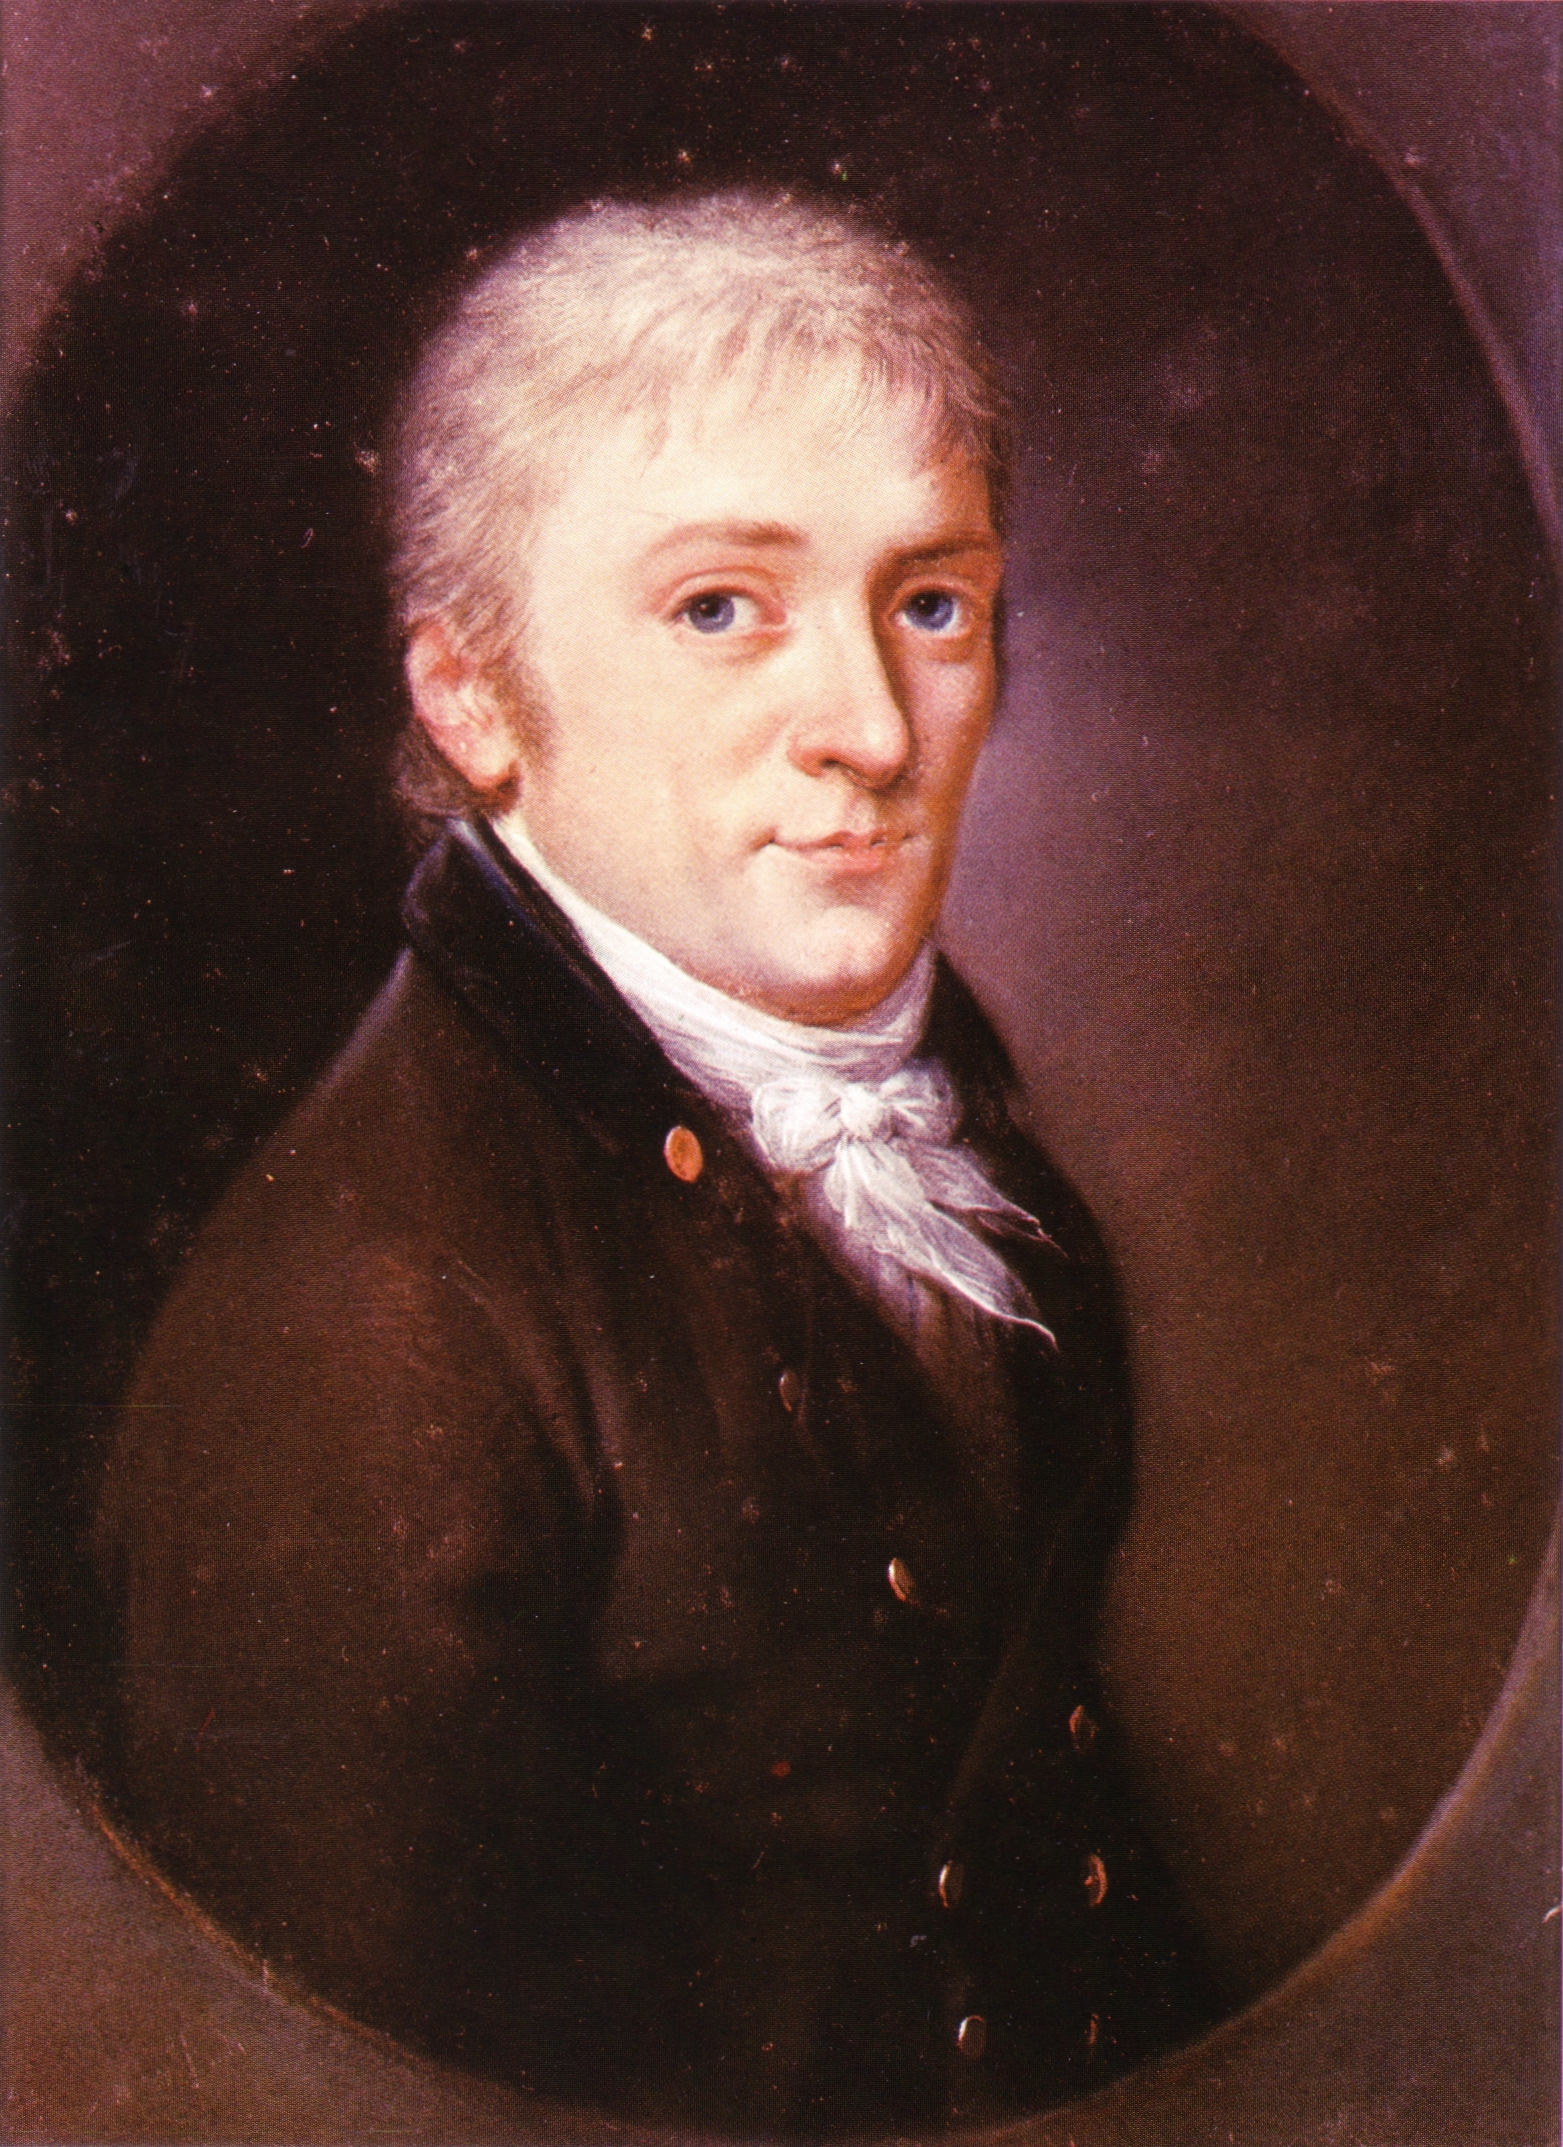
\includegraphics[width=0.32\textwidth]{gauss1803.jpg}%
    };
  \end{tikzpicture}
  \caption[Carl Friedrich Gauss]{\sloppy{Carl Friedrich Gauss. Pastel painting by Johann Christian August Schwartz, 1803.}}
  \label{figure:gauss-1803}
\end{figure}
\zcrefnamed{theorem:wilsons-theorem} can be used to prove a historically important result in the development of modular arithmetic: that $-1$ is congruent to a square modulo an odd prime $p$ if and only if $p\equiv 1\pmod{4}$.
In his \emph{Disquisitiones Arithmeticae} \cite{gauss1986}, Gauss writes of this result that when he encountered it in 1795---he was 19 at the time---he considered it to be a result of rare beauty and suspected deep connections with even
more profound results, that he concentrated all his efforts into understanding its underlying principles. He became so attracted by the questions of this nature, that he could not let them be. Ultimately, Gauss's investigations into higher arithmetic, as he preferred to call it, led him to prove the celebrated \zcrefnamed{theorem:quadratic-reciprocity}.

While the law of quadratic reciprocity is certainly the central theorem of our subject, the quadratic character of $-1$ modulo a prime is a key result on its own. In this section we will show that it can be used to show that there are infinitely many primes congruent to $1$ modulo $4$. Furthermore, we will use the fact that $-1$ is congruent to a square modulo $p$ when $p\equiv 1\pmod{4}$ in the next chapter to prove Fermat's \emph{Two-Square Theorem}, which asserts that every such prime is the sum of two squares. Questions similar to the quadratic character of $-1$ modulo a prime will be investigated more fully in \zcref{chapter:quadratic-residues,chapter:quadratic-reciprocity}.

\begin{theorem}[The Quadratic Character of $-1$]\label{theorem:quadratic-character-neg-1}
  Consider an odd prime $p$. Then there exists an integer $a$ such that
  \begin{equation*}
    a^2\equiv-1\pmod{p}
  \end{equation*}
  if and only if $p\equiv 1\pmod{4}$.
\end{theorem}

\begin{proof}
  First, we show that if there is an integer $a$ such that $a^2\equiv-1\pmod{p}$, then we must have $p\equiv 1\pmod{4}$. By \zcrefnamed{theorem:fermats-little-theorem} it follows that
  \begin{equation*}
    (-1)^{\frac{p-1}{2}}\equiv (a^2)^{\frac{p-1}{2}} \equiv a^{p-1}\equiv 1\pmod{p}
  \end{equation*}
  This shows that $\frac{p-1}{2}$ must be even, which is equivalent to the congruence $p\equiv 1\pmod{4}$.
  
  For the converse, assume that $p\equiv 1\pmod{4}$. By \zcrefnamed{theorem:wilsons-theorem} we know that $(p-1)!\equiv -1\pmod{p}$. Now, observe that the integers $1,\ldots,p-1$ can be arranged in pairs, where each $i$ is paired with $p-i$, which is always distinct from $i$ because $p-1$ is even. Since $i(p-i)\equiv -i^2\pmod{p}$, we obtain the congruences
  \begin{equation*}
    -1\equiv(p-1)!\equiv (-1)^{\frac{p-1}{2}}\left(\left(\frac{p-1}{2}\right)!\right)^2\equiv\left(\left(\frac{p-1}{2}\right)!\right)^2\pmod{p}.
  \end{equation*}
  The last congruence holds, because $(p-1)/2$ is even by the assumption that $p\equiv 1\pmod{4}$. Thus, we have presented $-1$ as a square modulo $p$.
\end{proof}

The previous theorem describing the quadratic character of $-1$ modulo an odd prime $p$ can be used to show that there are infinitely many primes congruent to $1$ modulo $4$. The first fifteen primes congruent to $1$ modulo $4$ are:
\begin{equation*}
  5,~13,~17,~29,~37,~41,~53,~61,~73,~89,~97,~101,~109,~113,~\text{and}~137.
\end{equation*}

\begin{theorem}
  There are infinitely many primes congruent to $1$ modulo $4$.
\end{theorem}

\begin{proof}
  Consider a finite set of primes $p_1,\ldots,p_k$ that are all congruent to $1$ modulo $4$, and define
  \begin{equation*}
    n = (2p_1\cdots p_k)^2 + 1.
  \end{equation*}
  Notice that $n\equiv 1\pmod{4}$ is greater than $1$, and $p_i\nmid n$ for any $1\leq i\leq k$. It follows that for any prime divisor $q$ of $n$, we have
  \begin{equation*}
    (2p_1\cdots p_k)^2\equiv -1\pmod{q},
  \end{equation*}
  showing that $-1$ is a quadratic residue modulo $q$. Since $-1$ is a quadratic residue modulo $q$ if and only if $q\equiv 1\pmod{4}$, it follows that any prime divisor $q$ of $n$ is congruent to $1$ modulo $4$. Since none of the prime divisors of $n$ are among the primes $p_i$ we started out with, the primes $p_i$ could not have listed all the primes congruent to $1$ modulo $4$.
\end{proof}

\zcref{theorem:quadratic-character-neg-1} and its proof can be generalized to arbitrary exponents. For example, the following theorem implies that the congruence $x^4\equiv -1\pmod{p}$ is solvable if and only if $p\equiv 1\pmod{8}$, that the congruence $x^8\equiv -1\pmod{p}$ is solvable if and only if $p\equiv 1\pmod{16}$, and so on.

\begin{theorem}
  Consider an odd prime $p$ and consider a natural number $n$ with $2$-adic decomposition $n=2^km$. Then the congruence
  \begin{equation*}
    x^n \equiv -1\pmod{p}
  \end{equation*}
  is solvable if and only if $p\equiv 1\pmod{2^{k+1}}$.
\end{theorem}

\begin{proof}
  The proof is by induction on $k$. For $k=0$, the statement is trivial, and for $k=1$, the proof was given in \zcref{theorem:quadratic-character-neg-1}. For the inductive step, assume that for any number $n$ with $2$-adic decomposition $n=2^km$, the congruence $x^n\equiv-1\pmod{p}$ is solvable if and only if $p\equiv 1\pmod{2^{k+1}}$, and consider a number $n$ with $2$-adic decomposition $n=2^{k+1}m$.

  For the forward direction, assume that $a$ is an integer such that $a^n\equiv -1\pmod{p}$. Then $b:=a^{2m}$ is an integer such that
  \begin{equation*}
    b^{2^k}\equiv -1\pmod{p},
  \end{equation*}
  so we see that $p\equiv 1\pmod{2^{k+1}}$. Consequently, the fraction
  \begin{equation*}
    \frac{p-1}{2^{k+1}}
  \end{equation*}
  is an integer. By \zcrefnamed{theorem:fermats-little-theorem} it follows that
  \begin{equation*}
    (-1)^{\frac{p-1}{2^{k+1}}}\equiv(a^{2^{k+1}m})^{\frac{p-1}{2^{k+1}}}\equiv (a^m)^{p-1}\equiv 1\pmod{p}.
  \end{equation*}
  This implies that $\frac{p-1}{2^{k+1}}$ is even, so that $p\equiv 1\pmod{2^{k+2}}$.

  For the converse, suppose that $p\equiv 1\pmod{2^{k+2}}$ and consider an integer $a$ such that $a^{2^k}\equiv -1\pmod{p}$. Such an integer exists by the inductive hypothesis. Now partition the set of numbers $\{1,\ldots,p-1\}$ into classes of $2^{k+1}$ numbers of the form $\{x,ax,\ldots,a^{2^{k+1}-1}x\}$. We will write $c$ for the number of such classes. Then we have $p=2^{k+1}c+1$, so we see that $c$ is even.

  Since the number of classes is $c$, we can label them by $C_i$ for each $1\leq i\leq c$, and we can pick a representative $x_i\in C_i$ for each $i$. Now it follows by \zcrefnamed{theorem:wilsons-theorem} that
  \begin{equation*}
    -1\equiv (p-1)!\equiv \prod_{i=1}^c \prod_{j=0}^{2^{k+1}-1} a^jx_i \equiv \prod_{i=1}^c (-1)x_i^{2^{k+1}} \equiv (-1)^c\prod_{i=1}^c x_i^{2^{k+1}} \equiv \left(\prod_{i=1}^c x_i\right)^{2^{k+1}}\pmod{p}.\qedhere
  \end{equation*}
\end{proof}

\section{The Infinitude of Primes Congruent to 1 Modulo Powers of 2}

One way to show that a prime $p$ is congruent to $1$ modulo $n$ is by finding an integer $a$ such that
\begin{equation*}
  \ord_p(a)=n.
\end{equation*}
By \zcrefnamed{theorem:order-theorem} and \zcrefnamed{theorem:fermats-little-theorem}, this implies that $n\mid p-1$. We will use this idea to show that there are infinitely many primes congruent to $1$ modulo any power of $2$. In particular, there are infinitely many primes congruent to $1$ modulo $4$, modulo $8$, modulo $16$, and so on.

\begin{theorem}\label{theorem:infinitude-of-primes-1-mod-power-of-2}
  For any positive natural number $n$, there are infinitely many primes congruent to $1$ modulo $2^n$.
\end{theorem}

\begin{proof}
  Since $p\equiv 1\pmod{2^{n+1}}$ implies that $p\equiv 1\pmod{2^n}$, it suffices to show that for any finite list $p_1,\ldots,p_k$ of primes congruent to $1$ modulo $2^{n+1}$, there is a prime $q\equiv 1\pmod{2^{n+1}}$ which is not among the primes $p_i$.

  Given such a list of primes $p_i$, let
  \begin{equation*}
    a:=2p_1\cdots p_k,
  \end{equation*}
  and let $q$ be a prime divisor of the integer $b:=a^{2^n}+1$. Note that $q$ is necessarily an odd prime, since $a$ is even and hence $b$ is odd. Since $p_i\nmid b$ for any $i$, it follows that $q$ is not among the primes $p_i$. Furthermore, we observe that
  \begin{equation*}
    a^{2^n}\equiv -1\pmod{q}.
  \end{equation*}
  This implies that $\ord_q(a)\mid 2^{n+1}$, while clearly $\ord_q(a)\nmid 2^n$. Thus, we must have $\ord_q(a)=2^{n+1}$, and this allows us to conclude that $q\equiv 1\pmod{2^{n+1}}$.
\end{proof}

The previous theorem is a special case of a deep theorem in analytic number theory: \emph{Dirichlet's Theorem}. Dirichlet's Theorem shows that for any integer $a$ relatively prime to $n$, there are infinitely many primes
\begin{equation*}
  p\equiv a\pmod{n}.
\end{equation*}
The techniques of proving Dirichlet's Theorem are beyond the scope of this course. However, having taken this course, you are well equipped to read LeVeque's excellent \emph{Topics in Number Theory} \cite{leveque1956vol1,leveque1956vol2}, a two-volume work that contains well-explained proofs of Dirichlet's Theorem as well as the Prime Number Theorem.

\exercises

\begin{starter}
  \exercise For every prime $p\equiv 1\pmod{4}$ below $100$, find the least positive integer $a$ such that $a^2\equiv -1\pmod{p}$.
  \exercise
  \begin{subexenum}
  \item Consider two integers $a$ and $b$, and a prime number $p$. Prove, without using Fermat's Little Theorem, that
    \begin{equation*}
      (a+b)^p\equiv a^p+b^p\pmod{p}.
    \end{equation*}
  \item Suppose that $a\geq 0$. Use the previous congruence and the fact that $a=\sum_{i=1}^a1$ to give your own proof of Fermat's Little Theorem.
  \end{subexenum}
  \exercise
  \begin{subexenum}
  \item Prove that
    \begin{equation*}
      5^{5^5}\equiv 5^5\pmod{31}.
    \end{equation*}
  \item Prove that
    \begin{equation*}
      7^{7^7}\equiv 7^7\pmod{43}.
    \end{equation*}
  \end{subexenum}
\end{starter}

\begin{routine}
  \exercise Show that
  \begin{equation*}
    2^{p-2}+3^{p-2}+6^{p-2} \equiv 1 \pmod{p}
  \end{equation*}
  for any prime number $p\neq 3$.
  \exercise For any positive integer $n$ we define the \emph{Euler quotient}
  \begin{equation*}
    q_n(x):=\frac{x^{\phi(n)}-1}{n},
  \end{equation*}
  where $x$ is assumed to be relatively prime to $n$. In the special case where $n$ is a prime, $q_n(x)$ is called the \emph{Fermat quotient}.
  \begin{subexenum}
  \item Show that
    \begin{equation*}
      q_n(ab)\equiv q_n(a)+q_n(b)\pmod{n}
    \end{equation*}
    for any two integers $a$ and $b$ relatively prime to $n$, and conclude that $q_n(a^k)\equiv k q_n(a)\pmod{n}$ for $a$ relatively prime to $n$.
  \item For any prime $p$, define the \emph{Wilson quotient} $W_p$ by
    \begin{equation*}
      W_p:=\frac{(p-1)!+1}{p}.
    \end{equation*}
    Prove \emph{Lerch's formula} \cite{lerch1905}, which asserts that
    \begin{equation*}
      \sum_{k=1}^{p-1}q_p(k)\equiv W_p\pmod{p}.
    \end{equation*}
  \end{subexenum}
  \exercise Show that
  \begin{equation*}
    3^{3^{3^3}}\equiv 3^{3^3}\pmod{97}.
  \end{equation*}
  \exercise
  \begin{subexenum}
  \item Show that any number of the form
    \begin{equation*}
      m^5n-n^5m
    \end{equation*}
    is divisible by $30$.
  \item Show that for any two odd primes $p$ and $q$, the number
    \begin{equation*}
      p^5q-q^5p
    \end{equation*}
    is divisible by $240$.
  \end{subexenum}
  \exercise Prove that if
  \begin{equation*}
    a^n\equiv a \pmod{n}
  \end{equation*}
  for every integer $a$, then $n=2$ or $n$ is odd.
  \exercise Consider two distinct primes $p$ and $q$, and an integer $a\geq 0$. Prove that
  \begin{equation*}
    a^{pq}+a\equiv a^p + a^q \pmod{pq}
  \end{equation*}
  \exercise Consider an odd prime $p=2n+1$. Show that
  \begin{equation*}
    \binom{2n}{n}\equiv (-1)^{\frac{p-1}{2}}\pmod{p}.
  \end{equation*}
  \exercise Consider a prime $p$ and two numbers $m$ and $n$. Prove that
  \begin{equation*}
    \binom{p^kn}{p^km}\equiv \binom{n}{m}\pmod{p}.
  \end{equation*}
  \exercise Show that the congruence
  \begin{equation*}
    \sum_{k=1}^{n} k^n\equiv 0\pmod{n}
  \end{equation*}
  holds if and only if $n$ is odd.
  \exercise
  \begin{subexenum}
  \item Consider a prime $p$ and an integer $p\nmid a$. Show that
    \begin{equation*}
      a^p\equiv a\pmod{p^2}\qquad\Leftrightarrow \qquad a^{p^2}\equiv a\pmod{p^2}.
    \end{equation*}
  \item A prime satisfying $a^p\equiv a\pmod{p^2}$ is called a \emph{Wieferich prime base $a$}. Wieferich encountered this condition by showing that if $x^p+y^p=z^p$ with $p\nmid xyz$, then $p$ must be a Wieferich prime base $2$ \cite{wieferich1909}. The only known Wieferich primes base $2$ are $p=1093$ and $p=3511$, and there are no smaller Wieferich primes base $2$.
    
    In bases larger than $2$ there are smaller Wieferich primes, although they are still rare. The only known Wieferich primes base $3$ are $p=11$ and $p=1006003$. Show that $5$ is a Wieferich prime base $32$.
  \end{subexenum}
\end{routine}

\begin{challenge}
  \exercise Find the least integer $k>1$ such that every integer of the form $x^k-x$ is divisible by $47$ and $89$.
  \exercise Find a prime $p>3$ such that
  \begin{equation*}
    3^{3^3}\equiv 3^3\pmod{p}.
  \end{equation*}
  \exercise For any integer $a$ and any prime number $p$, show that
  \begin{equation*}
    a^{p^k} \equiv a^{p^{k-1}} \pmod{p^k}.
  \end{equation*}
  \exercise Find all the solutions to the equation
  \begin{equation*}
    p^q-q^p=p+q,
  \end{equation*}
  where $p$ and $q$ are prime numbers.
  \exercise Consider two primes $p$ and $q$. Show that
  \begin{equation*}
    pq\mid (13^p-5^p)(13^q-5^q)\qquad\Leftrightarrow\qquad pq\mid 12.
  \end{equation*}
  \exercise
  \begin{subexenum}
  \item Show that the number $6481=3^8-3^4+1$ is prime. Hint: In order to avoid trying out all the primes below $80$, show first that every prime factor $p$ of $6481$ satisfies $p\equiv 1\pmod{24}$.
  \item Compute the prime factorization of the number
    \begin{equation*}
      3^{24}-1.
    \end{equation*}
  \end{subexenum}
  \exercise Consider the function $f(n)=2n+1$. Show for every prime $p$, the sequence
  \begin{equation*}
    k\mapsto f^k(p)
  \end{equation*}
  obtained by iterating the function $f$, contains composite numbers.
  \exercise \label{exercise:prime-divisors-feit-thompson-conjecture}
  \begin{subexenum}
  \item Consider an odd prime $q$. Show that the numbers
    \begin{equation*}
      2^q-1 \qquad\text{and}\qquad q+1.
    \end{equation*}
    are relatively prime.
  \item Consider two distinct primes $p$ and $q$, and let $r$ be a common prime divisor of the numbers
  \begin{equation*}
    \frac{p^q-1}{p-1}\qquad\text{and}\qquad\frac{q^p-1}{q-1}.
  \end{equation*}
  Show that $r\equiv 1\pmod{2pq}$.  
  \end{subexenum}
\end{challenge}

%%% Local Variables:
%%% mode: latex
%%% TeX-master: "elementary-number-theory"
%%% TeX-engine: luatex
%%% End:
